% (c) 2015 Daniele Zambelli daniele.zambelli@gmail.com

\chapter{Ellisse}

% \section{TODO}
% 
% \section{Ellisse con centro nell'origine e assi ...}
% \label{sec:01_formacanonica}

% \begin{wrapfloat}{figure}{r}{0pt}
% \includegraphics[scale=0.35]{img/fig000_.png}
% \caption{...}
% \label{fig:...}
% \end{wrapfloat}
% 
% \begin{center} \input{\folder lbr/fig000_.pgf} \end{center}

% \section{Altro paragrafo}
% \label{sec:ellisse_}

\section{Coniche}
\label{sec:ellisse_coniche}
  
  Le origini dello studio delle coniche si situano nel IV secolo a.C. 
in Grecia quando il matematico Menecmo scoprì le sezioni del cono nel 
tentativo di risolvere il problema della duplicazione del cubo. Nel III 
sec. a.C. Apollonio di Perge scrisse il più famoso trattato sull'argomento: 
``Coniche'' che in 8 libri raccoglie lo studio completo di questo 
argomento; in particolare Apollonio:
\begin{itemize} [nosep]
  \item conia i nomi di ellisse, parabola e iperbole per le 
tre sezioni;
  \item dimostra che tali sezioni sono ricavabili dall'intersezione tra un 
unico cono e un piano che  varia la sua inclinazione;
  \item dimostra quasi tutte le proprietà conosciute delle coniche.
\end{itemize}

\begin{figure}[htbp]
  \begin{minipage}{.75\textwidth}
Le coniche vengono dimenticate per quasi 1800 anni per 
venire riscoperte nel 1600 negli studi astronomici di Galilei, Newton e 
Keplero. La corrispondenza algebra-geometria di Cartesio consente di 
associare ad ogni conica un'equazione di secondo grado.
Entriamo nel merito geometrico. Per cono intendiamo il 
solido geometrico la cui superficie si ottiene facendo ruotare una retta r 
attorno ad una retta fissa detta asse di rotazione  che interseca r in un 
punto V, detto vertice. La superficie illimitata generata da r nella sua 
rotazione si dice superficie conica, con r generatrice e a asse di 
simmetria. Le due superfici, quella inferiore e quella superiore, cos\`{\i} 
generate prendono il nome di falde. L'angolo $ \alpha $ formato dalla 
generatrice con l'asse di rotazione si dice semiapertura della superficie 
conica.
  \end{minipage}
  \hspace{.5cm}
  \begin{minipage}{.20\textwidth}
  \begin{inaccessibleblock}[Cono a due falde tagliato da un piano
    che forma un'ellisse.]
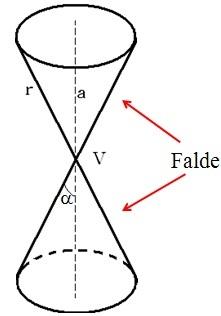
\includegraphics[height=3cm, width=3cm]{img/conoaduefalde.jpg}
    \caption{Cono a due falde.} 
\label{fig:conoaduefalde}
    \end{inaccessibleblock}
  \end{minipage}
\end{figure}
  
Come generiamo questo cono? Consideriamo una retta r nel piano e un asse di 
simmetria a verticale, facendo ruotare r  nello spazio, rispetto all'asse, 
otteniamo un cono a due falde:
\begin{figure}[htbp]
  \begin{inaccessibleblock}[Cono a due falde tagliato da un piano che forma 
un'ellisse.]
    \centering%
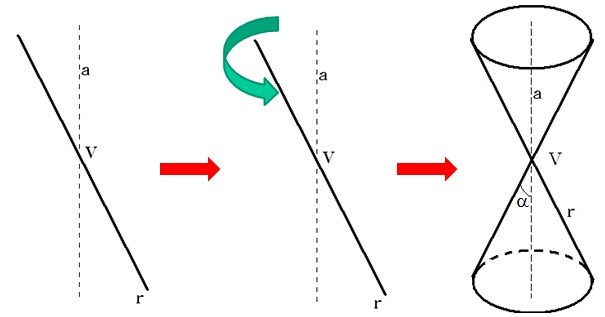
\includegraphics[height=7cm, width=7cm, keepaspectratio]{img/rotazionecono2.jpg}
    \caption{Generazione di un cono a due falde.}%
    %\label{fig:ellissedalcono}
  \end{inaccessibleblock}
\end{figure}

\subsection{Le sezioni coniche}  

Quando un piano interseca la superficie conica individua delle 
curve che prendono il nome di sezioni coniche. A seconda di come il piano 
taglia il cono, cioè con quale inclinazione, abbiamo quattro casi che 
illustriamo visivamente con la figura sottostante:  
  
\begin{figure}[htbp]
  \begin{inaccessibleblock}[Cono a due falde tagliato da un piano
    che forma un'ellisse.]
\centering%
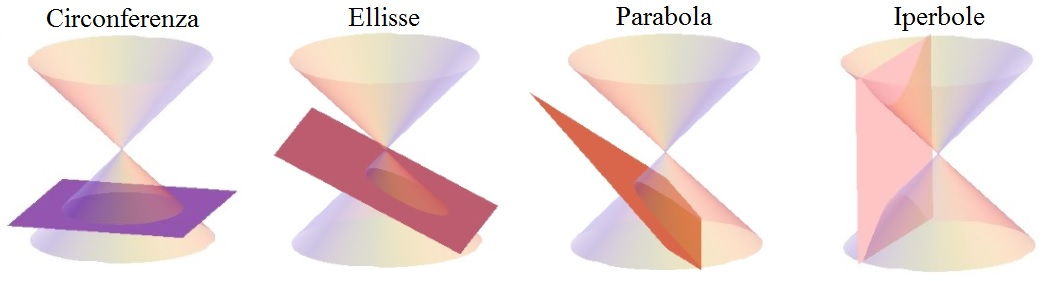
\includegraphics[height=8cm, width=13cm, keepaspectratio] {img/coniche.jpg}%
\caption{Le sezioni coniche.}%
\label{fig:coniche}
  \end{inaccessibleblock}  
\end{figure}

In particolare possiamo osservare i seguenti casi:

\begin{center}
\begin{tabular}{p{.3\textwidth} p{.3\textwidth} p{.3\textwidth}}
Se il piano è meno inclinato della generatrice rispetto ad 
una retta orizzontale, allora esso interseca una sola delle due falde del 
cono tagliando su di essa una curva chiusa detta ellisse. 
& 
Se il piano è parallelo alla generatrice, esso interseca 
una sola falda del cono e taglia su di essa una curva illimitata detta 
parabola. 
& 
Se il piano è più inclinato della generatrice esso 
interseca entrambe le falde del cono e taglia su di esse una curva spezzata 
in due rami, illimitata, detta iperbole. \\
\begin{center}
\begin{inaccessibleblock}[Cono a due falde tagliato da un piano
  che forma un'ellisse.]
  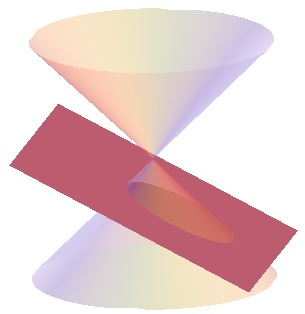
\includegraphics[height=2cm, width=2cm]{img/elisse2.jpg}
%   \caption{Generazione di un'ellisse.}
  \label{fig:elisse2}
\end{inaccessibleblock} 
\end{center}
& 
\begin{center}
\begin{inaccessibleblock}[Cono a due falde tagliato da un piano
  che forma una parabola.]
  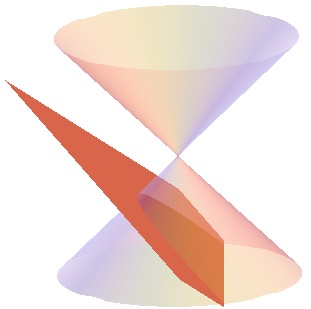
\includegraphics[height=2cm, width=2cm]{img/parabola3.jpg}
%   \caption{Generazione di una parabola.}
  \label{fig:parabola3}
\end{inaccessibleblock} 
\end{center}
&
\begin{center}
\begin{inaccessibleblock}[Cono a due falde tagliato da un piano
  che forma un'iperbole.]
  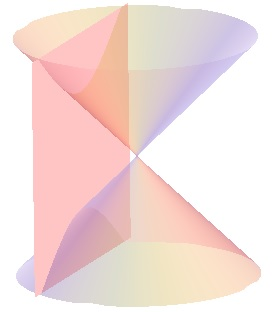
\includegraphics[height=2cm, width=2cm]{img/iperbole2.jpg}
%   \caption{Generazione di un'iperbole.} 
  \label{fig:iperbole2}
\end{inaccessibleblock}
\end{center}
\end{tabular}
\end{center}

Nel caso particolare che il piano sia perpendicolare all'asse del cono 
l'ellisse diventa una circonferenza. 

Studieremo le coniche nel piano cartesiano, ma come passare dallo spazio al 
piano? Il piano che taglia il cono a due falde è il nostro piano cartesiano e 
su di esso rimane impressa l'intersezione tra se stesso e la superficie del 
cono. Nelle figure \ref{fig:ellissedalcono} e \ref{fig:iperbolepiano} possiamo 
vedere la rappresentazione di questo passaggio per l'ellisse e per l'iperbole. 

\begin{figure}[htbp]
%    \begin{inaccessibleblock}[Cono a due falde tagliato da un piano
%      che forma un'ellisse.]
\centering%
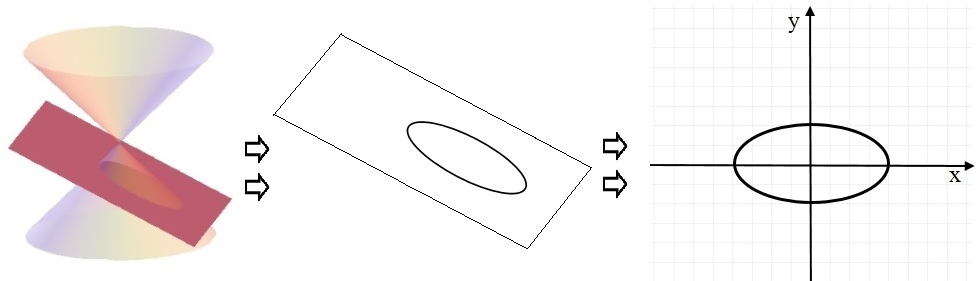
\includegraphics[height=8cm, width=14cm, keepaspectratio] 
{img/ellissedalcono.jpg}
\caption{L'ellisse da tre a due dimensioni.}
\label{fig:ellissedalcono}
%    \end{inaccessibleblock}
\end{figure}

\begin{figure}[htbp]
%    \begin{inaccessibleblock}[Cono a due falde tagliato da un piano
%      che forma un'ellisse.]
\centering%
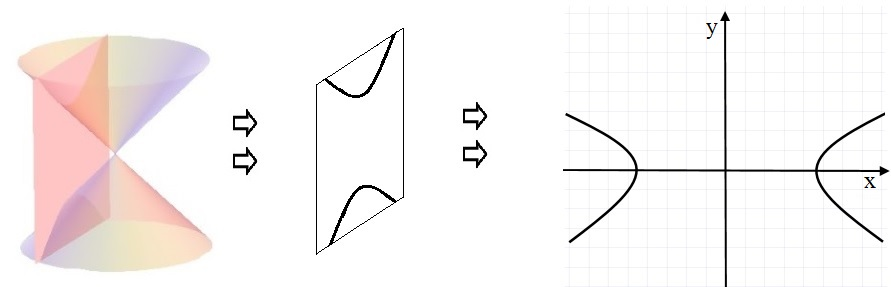
\includegraphics[height=8cm, width=14cm, keepaspectratio] 
{img/iperbolepiano.jpg}%
\caption{L'iperbole da tre a due dimensioni.}%
\label{fig:iperbolepiano}
%    \end{inaccessibleblock}
\end{figure}

Le coniche sono dunque l'insieme delle sezioni che una famiglia di piani 
stacca su una superficie conica a due falde, dal punto di vista della 
geometria in due dimensioni ciascuna delle 4 sezioni coniche può essere 
vista come luogo geometrico nel piano.

Potendo essere rappresentate sul piano come luogo geometrico, aventi quindi 
una determinata proprietà, le coniche possono essere interpretate da 
un'equazione algebrica. L'equazione generica delle coniche è un equazione 
di secondo grado in due variabili: 

\[ax^{2}+bxy+cy^{2}+dx+ey+f=0\] 

\section{L'ellisse}
\label{sec:ellisse_}

\noindent\begin{minipage}{.75\textwidth}
  L'ellisse è la conica corrispondente all'intersezione fra un cono a 
doppia falda e un piano quando il piano che taglia una delle due falde è 
meno inclinato della generatrice. La curva chiusa delineata dall'ellisse è 
una forma molto ricorrente nella vita quotidiana pensiamo solo alla forma 
di molte piazze o alla pianta di monumenti storici celeberrimi come il 
Colosseo a Roma. Le orbite dei pianeti del sistema solare ad esempio seguono 
una traiettoria ellittica.
\end{minipage}
\hspace{.5cm}
\begin{minipage}{.2\textwidth}
  %    \begin{inaccessibleblock}[Cono a due falde tagliato da un piano
  %      che forma un'ellisse.]
  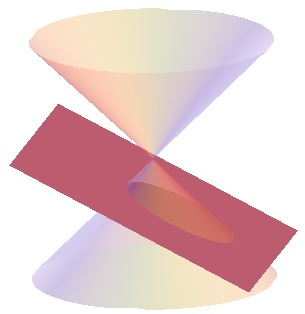
\includegraphics[width=\textwidth]{img/elisse2.jpg}
  %\caption{Generazione di un cono a due falde}% 
  %\label{fig:ellissedalcono}
  %    \end{inaccessibleblock}
\end{minipage} 

\subsection{L'ellisse come luogo geometrico}

L'ellisse può anche essere definita come un particolare insieme di punti:

\begin{definizione}
Dati nel piano $\pi$ due punti $F_{1}$ e $F_{2}$, detti fuochi, si 
dice ellisse E il luogo geometrico dei punti P di $\pi$ tali che sia 
costante la somma delle distanze di P da $F_{1}$ e $F_{2}$ 
\begin{equation}
%  E=\{P \in\pi~|~\overline{PF_{1}}+\overline{PF_{2}}=2a,a\in R_{+}^{0}\}
 E=\{P \in\pi \sand PF_{1}+PF_{2} = 2a,~2a \geqslant F_{1}F_{2}\}
\end{equation}
\end{definizione}

Leggiamo la formulazione della definizione. La somma delle distanze tra due 
punti definiti chiamati fuochi e un generico punto dell'ellisse risulta 
fissata e pari sempre a \(2a\), qualsiasi sia il punto dell'ellisse, come 
vediamo qui sotto per tre punti $P_{1}$, $P_{2}$ e $P_{3}$. Questa 
lunghezza, \(2a\), è associata ad un numero reale positivo diverso che non può 
essere minore della distanza tra i fuochi.

\begin{figure}[h]
  %    \begin{inaccessibleblock}[Cono a due falde tagliato da un piano
  %      che forma un'ellisse.]
  \centering
  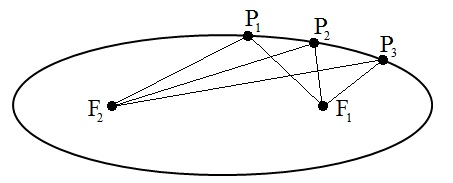
\includegraphics[height=8cm, width=6cm, keepaspectratio]
{img/ellissepunti.jpg}
  \caption{Costruzione di un'ellisse per punti.}%
  %\label{fig:ellissedalcono}
  %    \end{inaccessibleblock}
\end{figure}

Nella pratica possiamo ottenere una ellisse fissando le estremità di 
un filo di lunghezza 2a nei fuochi $ F_{1} $ ed $ F_{2} $, tra i quali c'è 
una distanza minore di 2a; quindi tenendo il filo ben teso si fa scorrere 
la punta della matita su un foglio come nella figura qui a sotto:
\begin{figure}[h]
  %    \begin{inaccessibleblock}[Cono a due falde tagliato da un piano
  %      che forma un'ellisse.]
  \centering%
  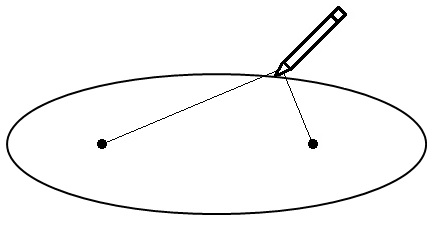
\includegraphics[height=8cm, width=6cm, keepaspectratio] {img/matita.jpg}%
  \caption{Costruzione di un'ellisse con filo e matita.}%
  %\label{fig:ellissedalcono}
  %    \end{inaccessibleblock}
\end{figure}

\begin{figure}[h]
\noindent\begin{minipage}{.50\textwidth}
Cerchiamo ora di descrivere questo luogo con una equazione. A partire alla 
definizione assegniamo le coordinate cartesiane ai due fuochi e al generico 
punto P: P(x; y), $ F_{1}(c;~0)$ e $ F_{2} (-c;~0)$, applichiamo poi la 
formula della distanza tra due punti in un piano cartesiano abbiamo:

\[\sqrt{(x+c)^{2}+y^{2}}+\sqrt{(x-c)^{2}+y^{2}}=2a\] 

con alcuni passaggi otteniamo l'espressione:
$\left( a^{2}-c^{2})x^{2}+a^{2}y^{2}=a^{2}(a^{2}-c^{2}\right)$
\end{minipage}
\hfill
\begin{minipage}{.48\textwidth}
\begin{center}
  %    \begin{inaccessibleblock}[Cono a due falde tagliato da un piano
  %      che forma un'ellisse.]
  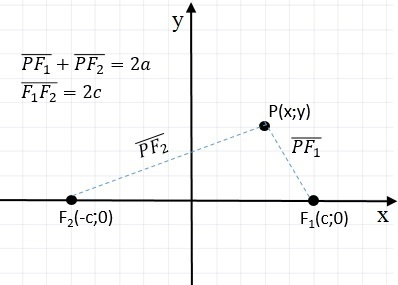
\includegraphics[width=.9\textwidth]{img/PF1F2.jpg}
  \caption{Ellisse come luogo geometrico.}
  %\label{fig:ellissedalcono}
  %    \end{inaccessibleblock}
\end{center}
\end{minipage} 
\end{figure}

Ora con la sostituzione $a^{2}-c^{2}=b^{2}$ otteniamo la più semplice:  
$b^{2}x^{2}+a^{2}y^{2}=a^{2}b^{2}$ che, dividendo entrambi i membri per 
$a^{2}b^{2}$, assume l'espressione:
\begin{equation}
\dfrac{x^{2}}{a^{2}}+\dfrac{y^{2}}{b^{2}}=1, \quad con  \quad a>b
\end{equation}

Questa espressione è detta equazione canonica o normale dell'ellisse.
Nel dettaglio abbiamo ottenuto l'equazione di un'ellisse coi fuochi 
appartenenti all'asse X.
Evidentemente nel caso particolare con a=b otteniamo $ x^{2}+y^{2}=a^{2}$, 
cioè una circonferenza con centro nell'origine e raggio a.

\subsection{Le caratteristiche dell'ellisse}

\begin{description}
\item [Intersezioni con gli assi]: vogliamo ora determinare le 
intersezioni dell'ellisse con gli assi cartesiani, per fare questo non 
dovremo fare altro che porre a sistema l'equazione dell'ellisse con le 
equazioni degli assi, prima y=0 e poi x=0.
\begin{figure}[h]
\hspace{8mm}
% \begin{minipage}{.1\textwidth}
% ~
% \end{minipage}
% \hfill
\begin{minipage}{.4\textwidth}
Le intersezioni relative all'asse X sono rispettivamente i punti:
$A_{1}(a;~0)$ e $A_{2}(-a;~0)$ mentre quelle relative all'asse Y sono:
$B_{1}(0;~b)$ e $B_{2}(0;~-b)$.

Questi quattro punti prendono il nome di vertici dell'ellisse. Risulta 
chiaro ora il significato dei parametri a e b, a è il semiasse maggiore 
dell'ellisse relativo alla sua dimensione maggiore, b è invece il semiasse 
minore dell'ellisse relativo alla sua dimensione minore. Chiaramente l'asse 
maggiore $\overline{A_{1}A_{2}}$ dell'ellisse avrà lunghezza 2a e giacerà 
sull'asse X mentre l'asse minore avrà lunghezza 2b e giacerà sull'asse Y, 
la distanza focale risulta evidentemente $\overline{F_{1}F_{2}}=2c$.
\end{minipage}
\hfill
\begin{minipage}{.53\textwidth}
\begin{center}
  %    \begin{inaccessibleblock}[Cono a due falde tagliato da un piano
  %      che forma un'ellisse.]
  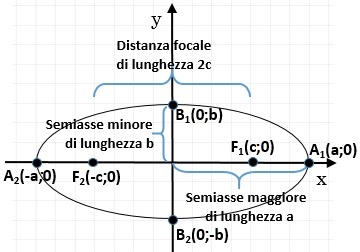
\includegraphics[width=.9\textwidth]{img/semiassi.jpg}
  \caption{Semiassi e distanza focale.}
  %\label{fig:ellissedalcono}
  %    \end{inaccessibleblock}
\end{center}
\end{minipage}
\end{figure}


\item [Simmetrie]: notiamo che l'ellisse, in cui l'intersezione tra i 
due assi è esattamente posta nell'origine, evidenzia una doppia simmetria, 
essendo simmetrica sia rispetto all'asse delle X che rispetto all'asse 
delle Y. Più propriamente ed in generale possiamo constatare che la 
proprietà di  simmetria dell'ellisse afferma che: la retta che congiunge i 
fuochi e l'asse del segmento $\overline{F_{1}F_{2}}$ assi di simmetria e il 
loro punto di intersezione è centro di simmetria dell'ellisse. 

\item [Limitazioni dell'ellisse]: essendo una curva chiusa possiamo 
facilmente stabilire i limiti a cui sono soggette le variabili 
caratterizzanti l'ellisse:
\[-a \leq x \leq a \qquad -b\leq y \leq b\]

\item [Relazioni tra i parametri]: ci chiediamo ora qual è la relazione 
tra i parametri visti cioè a semiasse maggiore, b semiasse minore e c 
ascissa del fuoco $ F_{1} $. Per ricavare questo non serve altro che 
rivedere come era stato identificato il parametro b quando abbiamo 
determinato l'equazione dell'ellisse. Esso era identificato come: 
\[a^{2} - c^{2} = b^{2}\]

\begin{minipage}{.7\textwidth}
  Con le formule inverse otteniamo dunque un parametro in funzione 
degli altri due:
\[a=\sqrt{b^{2}+c^{2}} \qquad \text{e} \qquad c=\sqrt{a^{2}-b^{2}}\]
  Dalla prima delle due precedenti formule otteniamo l'interessante 
proprietà che la distanza tra il punto di intersezione tra ellisse e asse 
minore e il fuoco è uguale ad a come mostra la figura a lato.
\end{minipage}
\hspace{.2cm}
\begin{minipage}{.25\textwidth}
  %    \begin{inaccessibleblock}[Cono a due falde tagliato da un piano
  %      che forma un'ellisse.]
  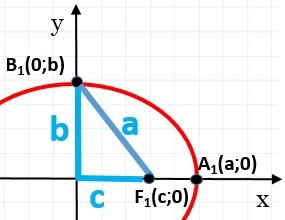
\includegraphics[width=\textwidth]{img/abc.jpg}
%   \caption{Relazione geometrica tra i parametri dell'ellisse.}
  %\label{fig:ellissedalcono}
  %    \end{inaccessibleblock}
\end{minipage}

% \begin{figure}[!h]
% \begin{minipage}{.7\textwidth}
%   Con le formule inverse otteniamo dunque un parametro in funzione 
% degli altri due:
% \[a=\sqrt{b^{2}+c^{2}} \qquad \text{e} \qquad c=\sqrt{a^{2}-b^{2}}\]
%   Dalla prima delle due precedenti formule otteniamo l'interessante 
% proprietà che la distanza tra il punto di intersezione tra ellisse e asse 
% minore e il fuoco è uguale ad a come mostra la figura qui a lato.
% \end{minipage}
% \hspace{.2cm}
% \begin{minipage}{.25\textwidth}
%   %    \begin{inaccessibleblock}[Cono a due falde tagliato da un piano
%   %      che forma un'ellisse.]
%   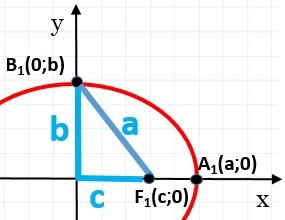
\includegraphics[width=\textwidth]{img/abc.jpg}
%   \caption{Relazione geometrica tra i parametri dell'ellisse.}
%   %\label{fig:ellissedalcono}
%   %    \end{inaccessibleblock}
% \end{minipage}
% \end{figure}

Le coordinate dei fuochi in funzione di a e b risultano:
\(F_{1} \punto{+\sqrt{a^{2}-b^{2}}}{0}\) e 
\(F_{2} \punto{-\sqrt{a^{2}-b^{2}}}{0}\)

\item [Eccentricità] il rapporto tra la distanza focale e la lunghezza 
dell'asse maggiore di un'ellisse è detto eccentricità e dell'ellisse
\begin{equation}
e=\dfrac{distanza \quad focale}{asse\quad 
maggiore}=\dfrac{2c}{2a}=\dfrac{c}{a}=\dfrac{\sqrt{a^{2}-b^{2}}}{a}
\end{equation}
Dato che \(c<a\) avremo che l'eccentricità \(e\):
\[0 \leq e leq 1\]
Vediamo cosa succede al variare dell'eccentricità tra 0 e 1.
Se e=0 la distanza focale è nulla, i due fuochi coincidono nel centro e 
quindi l'ellisse rappresenta una circonferenza di raggio a; se e$ > $0 la 
distanza focale è presente e separa i due fuochi che determinano uno 
schiacciamento sempre più marcato della precedente circonferenza, al 
crescere di e, che si schiaccia appunto sull'asse X; nel caso limite di e=1 
abbiamo che l'asse maggiore coincide con la distanza focale a=c e l'ellisse 
si appiattisce su un segmento di lunghezza pari a 2a=2c.
\begin{figure}[h]
  %    \begin{inaccessibleblock}[Cono a due falde tagliato da un piano
  %      che forma un'ellisse.]
  \centering%
  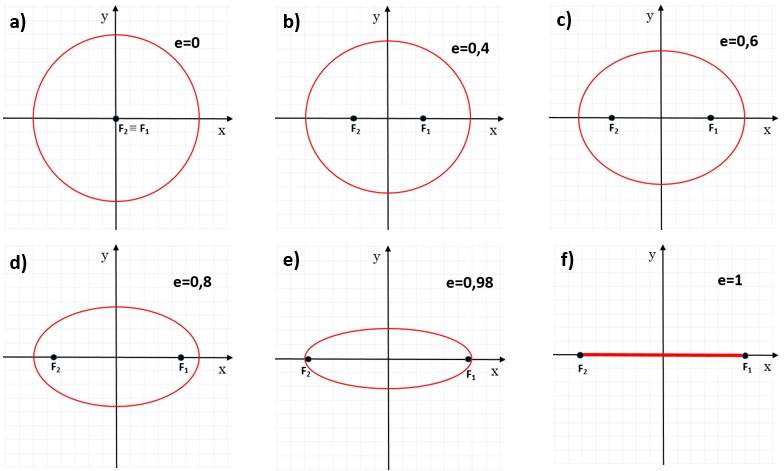
\includegraphics[height=9.2cm, width=9.2cm, keepaspectratio] 
{img/eccentricita.jpg}%
  \caption{Ellisse al variare dell'eccentricità. L'eccentricità pari 
a 0 nella figura a) corrisponde ad una circonferenza, mentre nella figura 
f) l'eccentricità pari a 1 schiaccia l'ellisse fino a farla diventare un 
segmento.}%
  %\label{fig:ellissedalcono}
  %    \end{inaccessibleblock}
\end{figure}
\end{description}

\begin{esempio}
Data l'ellisse$ \dfrac{x^{2}}{25} $+$ 
\frac{y^{2}}{16}=1 $ determinarne le caratteristiche e disegnarla.\\
$\Rightarrow$ Confrontando la formula dell'ellisse data con $ a^{2} $=25 e 
$ b^{2} $=16 da cui otteniamo i semiassi a=5 e b=4; i vertici dell'ellisse 
risultano quindi:
$ A_{1} (5;~0)$ e $ A_{2} (-5;~0)$,  $ B_{1} (0;~4)$ e $ B_{2} (0;~-4)$. \\
\begin{minipage}{.75\textwidth}
  Possiamo ora determinare la semidistanza focale c e 
conseguentemente i fuochi:\\ c=$ \sqrt{25-16} $=3, \qquad $ F_{1} (3;~0)$ e 
$ F_{2} (-3;~0)$. \\Infine l'eccentricità: e= $ \dfrac{3}{5} =~0,6$.
  il disegno dell'ellisse appena studiata è rappresentato qui a fianco
\end{minipage}
\hspace{0.5cm}
\begin{minipage}{.25\textwidth}
  %    \begin{inaccessibleblock}[Cono a due falde tagliato da un piano
  %      che forma un'ellisse.]
  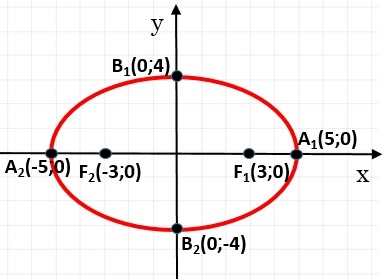
\includegraphics[width=\textwidth]{img/esempio1.jpg}
  %    \caption{Generazione di un cono a due falde}% 
  %\caption{Generazione di un'ellisse da un cono a due falde}
  %\label{fig:ellissedalcono}
  %    \end{inaccessibleblock}
\end{minipage}
\end{esempio}

\subsection{L'ellisse con i fuochi appartenenti all'asse Y}

% \begin{figure} [h]
\noindent \begin{minipage}{.75\textwidth}
   Se i fuochi dell'ellisse appartengono all'asse delle Y avremo 
un'ellisse che ha l'asse maggiore in senso verticale e quello minore in 
senso orizzontale, contrariamente all'ellisse appena vista. La somma delle 
distanze dai due fuochi sarà ora: $\overline{PF_{1}}+\overline{PF_{2}}=2b$ 
mentre i fuochi avranno coordinate $ F_{1} (0;~c)$ e $ F_{2} (0;~-c)$. 
L'equazione rimane:
  \begin{equation}
  \dfrac{x^{2}}{a^{2}}+\dfrac{y^{2}}{b^{2}}=1, \quad con  \quad a<b
  \end{equation}
  
\end{minipage}
 \hspace{0.5cm}
 \begin{minipage}{.2\textwidth}
   %    \begin{inaccessibleblock}[Cono a due falde tagliato da un piano
   %      che forma un'ellisse.]
   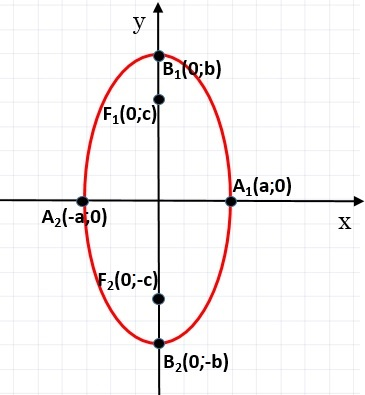
\includegraphics[width=\textwidth]{img/ellisseassey.jpg}
%    \caption{Ellisse con i fuochi sull'asse Y.}
   %\label{fig:ellissedalcono}
   %    \end{inaccessibleblock} 
\end{minipage}
% \end{figure}

Questa volta vale la relazione: $b^{2}-c^{2}=a^{2}$.

Le caratteristiche della nuova ellisse si possono ottenere con ragionamenti 
semplicemente simmetrici di scambio x-y rispetto alla precedente ellisse 
con fuochi sull'asse X; chiaramente ora l'asse maggiore sarà il segmento 
$\overline{B_{1}B_{2}}$      e l'asse minore il segmento 
$\overline{A_{1}A_{2}}$ .
Le nuove coordinate dei fuochi saranno:

Le coordinate dei fuochi risultano così subito dall'equazione canonica in 
funzione di a e b:

\(F_{1} \punto{0}{+\sqrt{a^{2}-b^{2}}}\) e 
\(F_{2} \punto{0}{-\sqrt{a^{2}-b^{2}}}\)

L'eccentricità invece, essendo ora \(2b\) l'asse maggiore sarà:

\begin{equation}
e=\dfrac{2c}{2b}=\dfrac{c}{b}=\dfrac{\sqrt{b^{2}-a^{2}}}{b}
\end{equation}

\subsection{Condizioni per determinare l'equazione dell'ellisse}

L'equazione di un'ellisse con centro di simmetria nell'origine e i fuochi 
su uno dei due assi cartesiani ha un'equazione dipendente dai due parametri 
a e b, occorrono dunque due condizioni per poter scrive l'equazione di una 
determinata ellisse.
Alcuni insiemi di condizioni che ci consentono di determinare l'ellisse 
sono i seguenti:
\begin{itemize} [noitemsep]
  \item passaggio dell'ellisse per due punti noti (non simmetrici tra 
loro rispetto a un asse cartesiano);
  \item conoscenza delle coordinate di un fuoco e un vertice;
  \item passaggio per un punto e conoscenza di un fuoco (o di un 
vertice);
  \item sono note le lunghezze dei semiassi;
  \item passaggio per un punto e si conoscenza dell'eccentricità;
  \item è nota l'eccentricità e si conoscono le coordinate di un 
fuoco (o di un vertice)
\end{itemize}

\begin{esempio}
Determinare l'equazione dell'ellisse avente a=11 e b=8.

$\Rightarrow$ Avendo i semiassi possiamo trovare i valori $ a^{2} $ e $ 
b^{2} $ presenti nella equazione 1.2 e ricostruire, con immediatezza, 
l'equazione dell'ellisse cercata:\quad $ 
\dfrac{x^{2}}{121}+\dfrac{y^{2}}{64}=1$
\end{esempio}

\begin{esempio}
Determinare l'equazione dell'ellisse 
avente e=$ \dfrac{3}{4} $ e $ F_{1} \left( \dfrac{3}{2} ;~0\right)$ .

$\Rightarrow$ Dall'ascissa del fuoco sappiamo che c=$ \dfrac{3}{2} $, ora 
dalla formula dell'eccentricità 1.3 ricaviamo a: $a= 
\dfrac{c}{e}=\dfrac{3}{2}\cdot\dfrac{4}{3}=2$. Dalle relazioni tra i 
parametri dell'ellisse sappiamo che 
$b=\sqrt{a^{2}-c^{2}}=\sqrt{4-\dfrac{9}{4}}=\sqrt{\dfrac{7}{4}}$.
L'equazione dell'ellisse cercata è dunque: $ 
\dfrac{x^{2}}{4}+\dfrac{4y^{2}}{7} =1$
\end{esempio}

\begin{esempio} 
 
Determinare l'equazione dell'ellisse 
passante per i punti:
\[P_{1} \punto{\sqrt{2}}{\sqrt{\dfrac{5}{2}}} \quad \text{e} \quad 
  P_{2} \punto{1}{\dfrac{\sqrt{15}}{2}}\]
Sostituiamo nell'equazione generica 1.2, le coordinate dei 
punti, ottenendo un sistema di due equazioni:
\[\sistema{\dfrac{2}{a^{2}}+\dfrac{5}{2b^{2}} =1   \\ \\ 
\dfrac{1}{a^{2}}+\dfrac{15}{4 b^{2}} =1 }\]
Il sistema sembra essere complesso in quanto sono 
presenti due variabili di secondo grado al denominatore. Per semplificarlo 
impostiamo questa sostituzione 
$t= \dfrac{1}{a^{2}} $ e $v= \dfrac{1}{b^{2}} $ 
e otteniamo il nuovo sistema:

\[\sistema{2t+\dfrac{5v}{2} =1 \\ \\ t+\dfrac{15v}{4} =1}\]
% \end{minipage}

Risolviamo il sistema ottenuto mediante la sostituzione

\vspace{6pt}
$\begin{cases}  2t+\dfrac{5v}{2} =1 \\ \\ t+\dfrac{15v}{4} =1  
\end{cases} \Rightarrow$ 
$\begin{cases}  2t+\dfrac{5v}{2} =1 \\  \\ t=-\dfrac{15v}{4} +1
\end{cases} \Rightarrow$
$\begin{cases}  2(-\dfrac{15v}{4}+1)+\dfrac{5v}{2}=1 \\ \\ t=-\dfrac{15v}{4} +1
\end{cases} \Rightarrow$
$\begin{cases}  -\dfrac{15v}{2}+2+\dfrac{5v}{2} =1 \\  \\ t=-\dfrac{15v}{4} +1 
\end{cases} \Rightarrow$

\vspace{6pt}
$\begin{cases}  -\dfrac{10v}{2} =-1 \\  \\ t=-\dfrac{15v}{4} +1  
\end{cases} \Rightarrow$
$\begin{cases}  v =\dfrac{1}{5}  \\ \\ t=-\dfrac{15}{4}\cdot\dfrac{1}{5} +1  
\end{cases} \Rightarrow$
$\begin{cases}  v =\dfrac{1}{5}  \\ \\ t=-\dfrac{3}{4} +1  
\end{cases} \Rightarrow$
$\begin{cases}  v =\dfrac{1}{5} \\  \\ t=\dfrac{1}{4}  
\end{cases}$

\vspace{6pt}
ora ricordando che t=$\dfrac{1}{a^{2}}$ e v=$\dfrac{1}{b^{2}}$
otteniamo l'ellisse cercata: 
$ \vspace{2cm} \dfrac{x^{2}}{4} + \dfrac{y^{2}}{5} = 1$
\end{esempio}

\begin{comment}
 
\section{L'iperbole}
\label{sec:iperbole_}

\noindent\begin{minipage}{.75\textwidth}
L'iperbole è la conica corrispondente all'intersezione fra un cono a doppia 
falda e un piano quando il piano essendo più inclinato della generatrice 
taglia entrambe le due falde del cono dando origine a una curva illimitata 
costituita da due parti dette rami.
\end{minipage}
\hspace{.5cm}
\begin{minipage}{.2\textwidth}
  %    \begin{inaccessibleblock}[Cono a due falde tagliato da un piano
  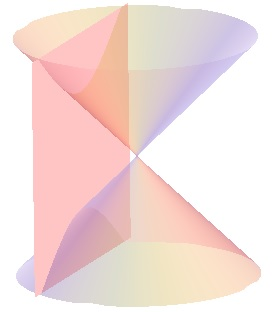
\includegraphics[width=\textwidth]{img/iperbole2.jpg}
  %    \caption{Generazione di un cono a due falde}% 
  %\label{fig:ellissedalcono}
  %    \end{inaccessibleblock}
\end{minipage}  

\subsection{L'iperbole come luogo geometrico}

Usando la sua proprietà di essere un particolare luogo geometrico del 
piano, possiamo definire l'iperbole come:
\begin{definizione}
  Dati nel piano $ \pi $ due punti $ F_{1} $ e $ F_{2} $, detti 
fuochi, si dice iperbole il luogo geometrico I dei punti P di $ \pi $ tali 
che sia costante la differenza delle distanze di P da $F_{1}$ e $F_{2}$ 

\begin{equation}
I=\{P \in\pi|\overline{PF_{1}}-\overline{PF_{2}}=2a,a\in R_{+}^{0}\}
\end{equation}
\end{definizione}
Leggiamo la formulazione della definizione. La differenza delle distanze 
tra due punti definiti chiamati fuochi e un generico punto P dell'iperbole 
risulta fissata e pari, sempre, a 2a, qualsiasi sia il punto dell'iperbole. 
Questa lunghezza, 2a, è associata ad un numero reale positivo diverso da 0.
\begin{figure}[h]
  %\hspace{12pt}
  \begin{minipage}[c]{.75\textwidth}
  I diversi punti P appartenenti al luogo geometrico dovranno dunque 
mantenere costante la differenza tra le lunghezze dei segmenti 
$\overline{PF_{1}}$ e $\overline{PF_{2}}$ come indicato nella figura a 
fianco:
  \end{minipage}
  \hspace{.5cm}
  \begin{minipage}[c]{.20\textwidth}
    %    \begin{inaccessibleblock}[Cono a due falde 
tagliato da un piano
    %      che forma un'ellisse.]
    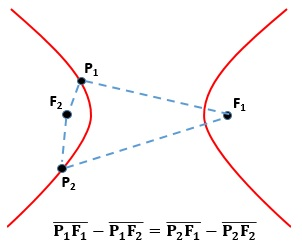
\includegraphics[width=\textwidth]{img/iperbol1.jpg}
    \caption{L'iperbole come luogo geometrico.}
    %\label{fig:ellissedalcono}
    %    \end{inaccessibleblock}
  \end{minipage}
\end{figure}

\begin{figure}[h]
  %\hspace{12pt}
  \begin{minipage}[c]{.75\textwidth}
  Cerchiamo ora di determinare l'equazione algebrica associata a 
questa curva.
    Consideriamo i due fuochi $ F_{1}(-c;~0)$ e $ F_{2}(0;~c)$ sull'asse 
delle X e chiamiamo il punto medio del segmento $\overline{F_{1}F_{2}}$ 
centro dell'iperbole con tale segmento $\overline{F_{1}F_{2}}$  detto 
distanza focale, pari a $\overline{F_{1}F_{2}} =2c$, mentre 2a è la 
distanza che deve rimanere costante per verificare il luogo geometrico in 
oggetto tale che sia valido: 
$\left|\overline{PF_{1}}-\overline{PF_{2}}\right|=2a$. 
  Utilizzando la formula per trovare la lunghezza di un segmento 
possiamo riscrivere il precedente modulo come:
    $\left|\sqrt{(x-c)^{2}+y^{2}} -\sqrt{(x+c)^{2}+y^{2}}\right|=2a$.
  \end{minipage}
  \hspace{.5cm}
  \begin{minipage}[c]{.2\textwidth}
    %    \begin{inaccessibleblock}[Cono a due falde 
tagliato da un piano
    %      che forma un'ellisse.]
    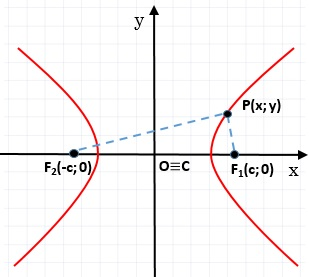
\includegraphics[width=\textwidth]{img/iperbol2.jpg}
    \caption{i fuochi dell'iperbole.}
    %\label{fig:ellissedalcono}
    %    \end{inaccessibleblock}
  \end{minipage}
\end{figure}
Sviluppando i calcoli come si è fatto per l'ellisse, con alcuni passaggi 
algebrici si ottiene l'espressione:\\
$\left( c^{2} -a^{2}\right) x^{2}+a^{2}y^{2}=a^{2}\left(c^{2}-a^{2}\right)$

Ora con la sostituzione $ c^{2}-a^{2}=b^{2} $ otteniamo la più semplice:  $ 
b^{2}x^{2}-a^{2}y^{2}=a^{2}b^{2}$  che dividendo entrambi i membri per $ 
a^{2}b^{2} $ assume l'espressione:
\begin{equation}
\dfrac{x^{2}}{a^{2}}-\dfrac{y^{2}}{b^{2}}=1
\end{equation}
detta equazione canonica dell'iperbole avente i fuochi sull'asse X.

\subsection{Le caratteristiche dell'iperbole}

\begin{description}
\item [Intersezioni con gli assi]: il grafico dell'iperbole, 
come abbiamo visto, interseca solo l'asse delle X in due punti $ A_{1} 
(a;~0)$ e $ A_{2}(-a;~0)$ le cui coordinate possono facilmente essere 
trovate risolvendo il sistema:

\centerline{$\begin{cases}  \dfrac{x^{2}}{a^{2}}-\dfrac{y^{2}}{b^{2}}=1   
\\ y =0  
  \end{cases}$$\Rightarrow$ $\begin{cases}  x=a  \\ y=0
  \end{cases}$}

Tali punti vengono detti vertici reali, l'asse che li congiunge, che 
coincide con X, è detto asse trasverso, mentre l'asse Y dove non vi sono 
intersezioni con l'iperbole viene detto asse non trasverso.\\
\item [Simmetrie dell'iperbole]: dato che nell'equazione canonica sia 
la variabile x che la variabile y appaiono di secondo grado se P (x, y) è 
un generico punto dell'iperbole anche i punti $ P_{1}(-x;~y)$,     $ 
P_{2}(-x;~-y)$ e $ P_{3}(x;~-y)$ appartengono all'iperbole e possiamo 
affermare dunque che l'iperbole è una curva simmetrica rispetto all'asse X, 
rispetto all'asse Y e rispetto all'origine.\\
\item [Vertici non reali, asintoti e la costruzione dell'iperbole]:
 abbiamo appena mostrato che il parametro a ci dà le ascisse dei  punti di 
intersezione dell'iperbole con l'asse delle X, possiamo affermare qualcosa 
di simile per il parametro b? Sicuramente non nella stessa forma, in quanto 
l'iperbole non ha intersezioni con l'asse Y. 
\begin{figure}[h]
  %\hspace{12pt}
  \begin{minipage}[c]{.75\textwidth}
  Tuttavia risulta comodo definire, parallelamente ai due vertici 
reali, altri due vertici, stavolta non reali sull'asse delle Y: i punti $ 
B_{1} (0; b)$ e $ B_{2} (0; -b)$. Non reali in quanto non identificano una 
intersezione reale.\\ Costruiamo ora un rettangolo di lati 2a e 2b con i 
punti $ A_{1} $, $ A_{2} $, $ B_{1} $ e $ B_{2} $, punti medi di tali lati: 
il segmento che congiunge l'origine ad uno dei vertici risulta lungo c, da 
quanto visto nella determinazione dell'equazione dell'iperbole infatti $ 
c^{2} = a^{2} + b^{2} $.
  \end{minipage}
  \hspace{.5cm}
  \begin{minipage}[c]{.2\textwidth}
    %    \begin{inaccessibleblock}[Cono a due falde 
tagliato da un piano
    %      che forma un'ellisse.]
    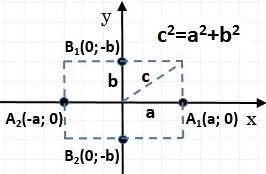
\includegraphics[width=\textwidth]{img/rettangolo.jpg}
    \caption{Relazione tra i parametri dell' iperbole.}
    %\label{fig:ellissedalcono}
    %    \end{inaccessibleblock}
  \end{minipage}
\end{figure}

Cerchiamo di capire la relazione tra il rettangolo appena determinato e 
l'iperbole.\\ \\ \\ \\  \\ \\ \\ \\
\begin{figure}[h]
  %\hspace{12pt}
  \begin{minipage}[c]{.65\textwidth}
    L'iperbole tocca il rettangolo $ A_{1} $$ A_{2} $$ B_{1} $$ 
B_{2} $ soltanto nei vertici reali $ A_{1} $ e $ A_{2} $ e si sviluppa 
illimitatamente all'interno delle due parti di piano delimitate da due 
rette, chiamate asintoti. Gli asintoti non sono altro che la prosecuzione 
delle diagonali del rettangolo ed hanno come coefficiente angolare m=$ \pm 
$b/a. Gli stessi asintoti forniscono una sorta di limite ne valicabile ne 
raggiungibile da parte dell'iperbole. Le equazioni di queste rette, 
passanti per l'origine sono y=$ \dfrac{b}{a} $ e y=-$ \dfrac{b}{a} $.
  \end{minipage}
  \hspace{.2cm}
  \begin{minipage}[c]{.3\textwidth}
    %    \begin{inaccessibleblock}[Cono a due falde 
tagliato da un piano
    %      che forma un'ellisse.]
    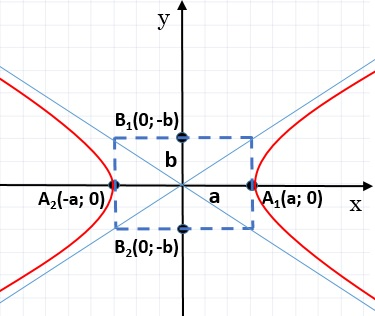
\includegraphics[width=\textwidth]{img/asintoti.jpg}
    \caption{il rettangolo caratteristico dell'iperbole.}
    %\label{fig:ellissedalcono}
    %    \end{inaccessibleblock}
  \end{minipage}
\end{figure}

Notiamo infine che possiamo esprimere le coordinate dei fuochi in funzione 
di a e b come: $ F_{1}(\sqrt{a^{2}+b^{2}}, 0) $, $ 
F_{2}(-\sqrt{a^{2}+b^{2}}, 0) $
\item [Eccentricità] Analogamente a 
quanto visto per l'ellisse definiamo l'eccentricità di un iperbole quel 
valore pari al rapporto tra distanza focale e lunghezza dell'asse trasverso:
\begin{equation}
e=\dfrac{distanza \quad focale}{lunghezza \quad asse\quad 
trasverso}=\dfrac{2c}{2a}=\dfrac{c}{a}=\dfrac{\sqrt{a^{2}+b^{2}}}{a}
\end{equation}
poiché dalla precedente formula c>a osserviamo che e>1.
Per comprendere il significato geometrico dell'eccentricità e notare come 
al suo variare cambi il grafico dell'iperbole, studiamo come cambia 
l'eccentricità al variare di b tenendo fissa a, con i seguenti esempi:
\begin{figure}[htbp]
  \centering
  %    \begin{inaccessibleblock}[Cono a due falde tagliato da un piano
  %      che forma un'ellisse.]
  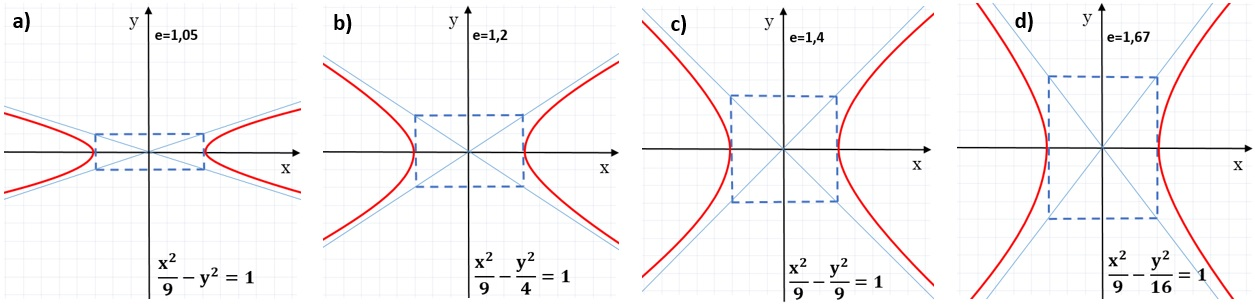
\includegraphics[width=\textwidth]{img/4iperboli.jpg}
    \caption{Eccentricità dell'iperbole al variare del 
parametro b.}%
  %\label{fig:ellissedalcono}
  %    \end{inaccessibleblock}
\end{figure}
\end{description}

\subsection{L'iperbole con i fuochi sull'asse Y}

Se i fuochi, al contrario di quanto visto finora, giacciono sull'asse Y e 
hanno coordinate $ F_{1} (0;~-c)$ e $ F_{2} (0;~c)$ prende forma una nuova 
tipologia di iperbole che invece di svilupparsi a sinistra e a destra 
dell'origine si sviluppa sopra e sotto di tale punto.
Con ragionamenti molto simili ai precedenti partendo stavolta dalla: 
$\left|\overline{PF_{1}}-\overline{PF_{2}}\right|=2b$ riusciamo a 
determinare l'equazione canonica di questo tipo di iperbole che è: 
\begin{equation}
\dfrac{x^{2}}{a^{2}}-\dfrac{y^{2}}{b^{2}}=-1
\end{equation}
Si può poi verificare che:
\begin{itemize}
  \item l'iperbole è simmetrica rispetto all'origine e agli assi 
cartesiani ;
  \item l'asse Y è l'asse trasverso e su di esso giacciono i vertici 
reali $ B_{1} (0;~b)$ e $ B_{2} (0;~-b)$;
  \item l'asse X è l'asse non trasverso dove giacciono i vertici non 
reali $ A_{1} (a;~0)$ e $ A_{2} (-a;~0)$;
  \item le rette di equazione y=$ \dfrac{b}{a} $ x  e   
$y=-\dfrac{b}{a} x$ sono gli asintoti dell'iperbole ;
  \item è definita l'eccentricità 
$e=\dfrac{c}{b}=\dfrac{\sqrt{b^{2}+a^{2}}}{b} $
\end{itemize}

\subsection{Condizioni per determinare l'equazione dell'iperbole}

Similmente a quanto visto per l'ellisse, essendo anche l'iperbole 
determinata da due parametri, a e b, serviranno solo due condizioni per 
trovarne l'equazione completa e caratterizzante.
Le coppie di informazioni che insieme consentono di determinare un'iperbole 
sono:
\begin{itemize}
\item la conoscenza di due punti dell'iperbole, non simmetrici rispetto 
agli assi o rispetto all'origine;
\item la conoscenza di un punto e un fuoco (o un vertice);
\item sono noti un fuoco e un vertice;
\item la conoscenza dell'eccentricità e di un fuoco, o di un vertice, o di 
un punto dell'iperbole;
\item la conoscenza di un asintoto e di un fuoco, o un vertice o un punto 
dell'iperbole.
\end{itemize}

\subsection{L'iperbole equilatera e la funzione omografica}

Se le lunghezze dei semiassi trasverso e non trasverso sono uguali, a=b, 
l'equazione dell'iperbole diventa: 
$ \dfrac{x^{2}}{a^{2}}-\dfrac{y^{2}}{a^{2}}=1$,   equivalente a   $ 
x^{2}-y^{2} $=$ a^{2} $. 
Tale forma di iperbole, con un solo parametro è detta 
\emph{iperbole equilatera riferita ai propri assi}. 
In questo caso gli altri elementi che caratterizzano l'iperbole diventano:

\begin{figure}[h]
  %\hspace{12pt}
  \begin{minipage}[c]{.65\textwidth}
  \begin{itemize}
    \item gli asintoti sono $y=x$ e $y=-x$ cioè le bisettrici 
dei quadranti;
    \item la semidistanza focale c diventa c=a$ \sqrt{2} $;
    \item l'eccentricità è e=$ 
\dfrac{\sqrt{a^{2}+a^{2}}}{a}=\sqrt{2} $
    \item   i fuochi sono $ F_{1} \left(a \sqrt{2};~0\right)$ e 
$ F_{2}\left(-a \sqrt{2};~0\right)$
    \item i vertici reali sono $ A_{1}(a;~0)$e $ 
A_{2}(-a;~0)$  
  \end{itemize}    
  \end{minipage}
  \hspace{.2cm}
  \begin{minipage}[c]{.3\textwidth}
    %    \begin{inaccessibleblock}[Cono a due falde 
tagliato da un piano
    %      che forma un'ellisse.]
    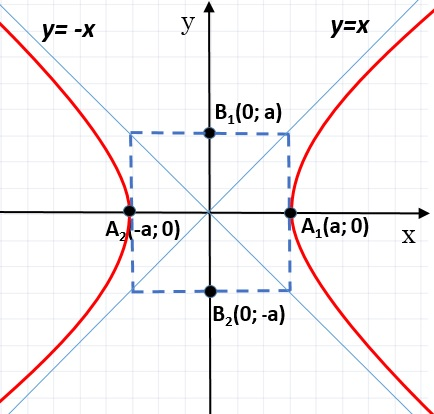
\includegraphics[height=4cm, width=4cm,]{img/equilatera.jpg}
    \caption{L'iperbole equilatera.}
    %\label{fig:ellissedalcono}
    %    \end{inaccessibleblock}
  \end{minipage}
\end{figure}
\begin{itemize}
  \item il rettangolo che prima caratterizzava l'iperbole diventa ora 
un quadrato di lato 2a 
\end{itemize}

\noindent Nel caso simmetrico in cui i fuochi appartengono all'asse Y 
l'equazione diventa: $ x^{2} - y^{2} =- a^{2} $, con i fuochi  $ F_{1} 
\left(0; a \sqrt{2}\right)$, $ F_{2} \left(0;~-a \sqrt{2}\right)$ e vertici 
reali $ B_{1} (0; a)$,$ B_{2} (0; -a)$.
Se ruotiamo di $45^\circ$ gradi l'iperbole equilatera riferita ai propri 
assi otteniamo una nuova iperbole che ha come asintoti gli assi cartesiani 
e come assi di simmetria le bisettrici dei quadranti, chiamiamo questo tipo 
di iperbole: \emph{iperbole equilatera riferita ai propri asintoti}.

Si può dimostrare che l'equazione di tale iperbole si può scrivere nella 
forma: 
\begin{equation}
x\cdot y=k \hspace{1cm} con \hspace{0.2cm}k \neq 0
\end{equation}
nel dettaglio a seconda del segno di k abbiamo: 
\begin{figure}[htbp]
  \centering
  %    \begin{inaccessibleblock}[Cono a due falde tagliato da un piano
  %      che forma un'ellisse.]
  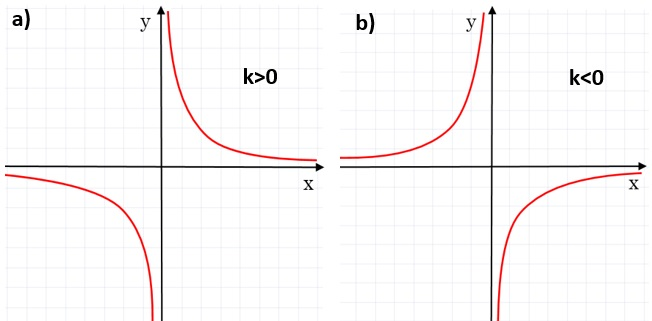
\includegraphics[height=8cm, width=14cm]{img/equilatera2.jpg}
  \caption{Iperbole equilatera con k>0 e k<0.}
  %\label{fig:ellissedalcono}
  %    \end{inaccessibleblock}
\end{figure}

Notiamo che l'equazione xy=k non è altro che l'espressione della 
proporzionalità inversa tra due grandezze che mantengono costante il loro 
prodotto e k è la loro costante di proporzionalità. Soffermiamoci sulla 
figura 10a, i vertici di questa iperbole, utili per disegnarla, sono dati 
dall'intersezione dell'iperbole con la bisettrice del primo e terzo 
quadrante. Mettendo a sistema xy=k e x=y otteniamo che i vertici sono $ 
A_{1} \left( \sqrt{k} ,~\sqrt{k} \right)$ e $ A_{2} \left(- \sqrt{k},~- 
\sqrt{k} \right)$.

Vi è, poi, un'altra importante scrittura che rappresenta un'iperbole 
equilatera, una funzione matematica che viene rappresentata nel piano come 
un'iperbole traslata rispetto all'origine.
Tale funzione, detta \emph{funzione omografica} è data dalla curva 
di equazione:
\begin{equation}
y= \dfrac{ax+b}{cx+d} \qquad con \quad a,b,c,d\in \textbf{R},\quad c\neq0 
\quad e \quad ad-bc \neq 0
\end{equation}
La funzione appena trovata è un'iperbole equilatera che ha come asintoti le 
rette $y= \dfrac{a}{c} $ e $x=-\dfrac{d}{c}$ e come centro di simmetria il 
punto C $\left( -\dfrac{d}{c};~\dfrac{a}{c}\right)$.\\ \\  
\begin{figure}%[htbp]
  \centering
  %    \begin{inaccessibleblock}[Cono a due falde tagliato da un piano
  %      che forma un'ellisse.]
  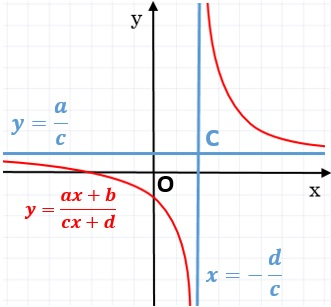
\includegraphics[height=8cm, width=8cm]{img/omografica.jpg}
  \caption{Funzione omografica.}%
  %\label{fig:ellissedalcono}
  %    \end{inaccessibleblock}
\end{figure}
Cerchiamo di capire meglio il significato delle due condizioni 
precedentemente poste nell'equazione della funzione omografica:

\begin{itemize}
  \item se c= 0 otteniamo $y= \dfrac{ax+b}{d} $ cioè $y= 
\dfrac{ax}{d} + \dfrac{b}{d} $, che rappresenta una semplice retta;
  \item se $ad-bc=0$, cioè $ \dfrac{d}{c} = \dfrac{b}{a} $, 
l'equazione si può scrivere nella forma:
y= $\dfrac{ax+b}{cx+d}=  \dfrac{a\left(x+ \frac{b}{a} \right)}{c\left(x+ 
\frac{d}{c} \right)} $ da cui, per $x \neq -\dfrac{d}{c} $, abbiamo y=$ 
\dfrac{a}{c} $; cioè, se $ad-bc=0$ otteniamo una retta di equazione y=a/c 
definita per tutte le x escluso il valore $x=-d/c$.  
\end{itemize}

\begin{esempio}
\begin{figure}[h]
  %\hspace{12pt}
  \begin{minipage}[c]{.65\textwidth}
    Data l'iperbole equilatera $ x^{2} - y^{2} =6$, determina i 
vertici i fuochi e c, infine disegnala.\\
    Poiché $a= \sqrt{6} $, i vertici risultano $ A_{1} 
\left(\sqrt{6};~ 0\right)$ e $ A_{2} \left(-\sqrt{6};~ 0\right)$ e $c= 
\sqrt{6}  \sqrt{2} = \sqrt{12} =2 \sqrt{3} $. Dalla conoscenza di c 
otteniamo i fuochi $ F_{1} \left(2\sqrt{3};~ 0\right)$ e $ F_{2} 
\left(-2\sqrt{3}; ~0\right)$.
    
  \end{minipage}
  \hspace{.2cm}
  \begin{minipage}[c]{.25\textwidth}
    %    \begin{inaccessibleblock}[Cono a due falde tagliato da un piano
    %      che forma un'ellisse.]
    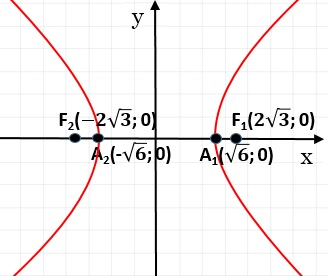
\includegraphics[width=\textwidth]{img/equilatera1.jpg}
    %\caption{Generazione di un'ellisse da un cono a due falde}
    %\label{fig:ellissedalcono}
    %    \end{inaccessibleblock}
  \end{minipage}
\end{figure}
\end{esempio}

\begin{esempio}
\begin{figure}[h]

  %\hspace{12pt}
  \begin{minipage}[c]{.65\textwidth}
    Data l'iperbole equilatera $xy=8$, determina i suoi vertici 
e disegnala.\\ Si tratta di un'iperbole equilatera riferita ai propri 
asintoti e poiché k> 0 si trova nel primo e nel terzo quadrante. I vertici 
sono: $ A_{1} \left(2\sqrt{2}; 2\sqrt{2}\right)$ e $ A_{2} 
\left(-2\sqrt{2}; -2\sqrt{2}\right)$
    
  \end{minipage}
  \hspace{.2cm}
  \begin{minipage}[c]{.25\textwidth}
    %    \begin{inaccessibleblock}[Cono a due falde tagliato da un piano
    %      che forma un'ellisse.]
    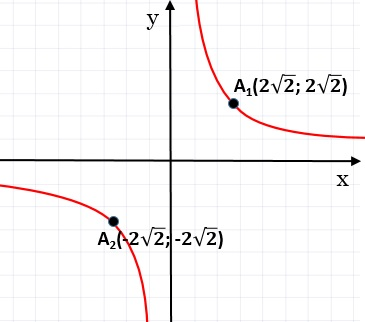
\includegraphics[width=\textwidth]{img/equilatera2a.jpg}
    %\caption{Generazione di un'ellisse da un cono a due falde}
    %\label{fig:ellissedalcono}
    %    \end{inaccessibleblock}
  \end{minipage}
\end{figure}
\end{esempio}

\begin{esempio} Data la funzione omografica y=$ 
\dfrac{x-3}{x+2} $ dopo aver verificato che è un'iperbole , determinane gli 
asintoti e il centro di simmetria. Completa l'esercizio facendo il disegno 
della funzione.\\Per verificare se si tratta di un iperbole constatiamo che 
c=1, quindi c$ \neq $0 e poi calcoliamo $ad-bc$. Se questa espressione è 
diversa da 0 la funzione omografica rappresenta una iperbole: $ad-bc=5$. 
Possiamo ora determinare gli asintoti, quello verticale è 
$x=- \dfrac{d}{c} =-2$ e quello orizzontale è $y= \dfrac{a}{c} =1$; 
il centro di simmetria è $C(-2; ~1)$.

\begin{figure}[h]
  %\hspace{12pt}
  \begin{minipage}[c]{.65\textwidth}
     Per disegnare la funzione dobbiamo avere i riferimenti dei 
punti in cui il grafico interseca gli assi, per trovare quella con l'asse X 
basta risolvere il sistema tra la funzione e x=0, per determinare quella 
con Y basta risolvere il sistema tra l'equazione e y=0. i due punti cercati 
sono $ P_{1}  \left(0;~ - \dfrac{3}{2} \right)$ e $ P_{2} =(3;~0)$.
    
  \end{minipage}
  \hspace{.2cm}
  \begin{minipage}[c]{.25\textwidth}
    %    \begin{inaccessibleblock}[Cono a due falde tagliato da un piano
    %      che forma un'ellisse.]
    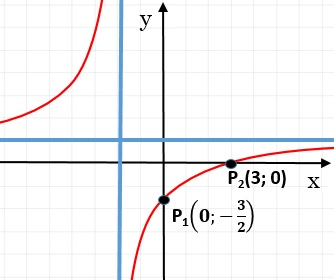
\includegraphics[width=\textwidth]{img/equilatera2b.jpg}
    %\caption{Generazione di un'ellisse da un cono a due falde}
    %\label{fig:ellissedalcono}
    %    \end{inaccessibleblock}
  \end{minipage}
\end{figure}
\end{esempio}

\end{comment}
% 
% \section{Esercizi}
% 
% \subsection{Esercizi dei singoli paragrafi}

\begin{comment}
 

L'iperbole come luogo geometrico.
\begin{esercizio}
  \label{ese:div.003}
  Considera gli elementi dati nelle iperboli sottostanti e scrivine 
l'equazione.
\begin{figure}[htbp]
  \centering%
  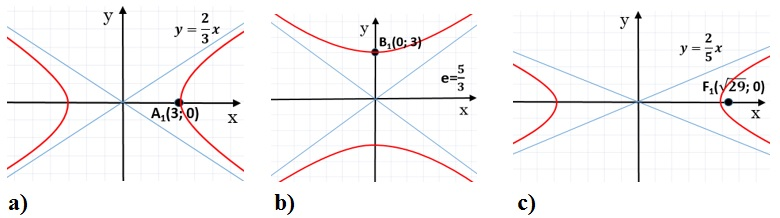
\includegraphics[height=16cm, width=12cm, keepaspectratio] 
{img/graficiip.jpg}%
  %\caption{Generazione di un cono a due falde}%
\end{figure}
\end{esercizio}
\noindent Le caratteristiche dell'iperbole.\\
\begin{esercizio}
  \label{ese:div.003}
  Determina le misure del semiasse trasverso, del semiasse non 
trasverso e i fuochi delle seguenti iperboli.
  \begin{enumeratea}
  \item $ \dfrac{x^{2}}{25} - \dfrac{y^{2}}{16} =1$
  \hfill $\left[a=5;~ b=4;~ F_{1} \left( \sqrt{41} ;~ 0\right), ~ 
F_{2}  \left(- \sqrt{41} ;~0\right)\right]$
  \item $ \dfrac{x^{2}}{4} - \dfrac{y^{2}}{9} =1$
  \hfill $\left[a=2; ~b=3; ~ F_{1} \left( \sqrt{13} ;~ 0\right), ~ 
F_{2}  \left(- \sqrt{13} ;~ 0\right)\right]$
  \item $ \dfrac{x^{2}}{11} - \dfrac{y^{2}}{5} =1$
  \hfill $\left[a= \sqrt{11} ;~ b= \sqrt{5} ;~  F_{1}  (4; 0), ~ 
F_{2}  (-4; 0)\right]$
  \item $ \dfrac{x^{2}}{16} - \dfrac{y^{2}}{9} =1$
  \hfill   \
    $\left[a=4; b=3; ~ F_{1}  (5 ; 0), ~ F_{2}  (-5 ; 0)\right]$
  \item $ 25x^{2} - 4y^{2} =100$
  \hfill $\left[a=2;~ b=5; ~ F_{1} \left( \sqrt{29} ; ~0\right), ~ 
F_{2}  \left(- \sqrt{29} ;~ 0\right)\right]$
  \item $ x^{2} - y^{2} =49$
  \hfill $\left[a=7;~ b=7; ~ F_{1}  \left(7 \sqrt{2} ; ~0\right),  
F_{2}  \left(-7 \sqrt{2} ;~ 0\right)\right]$
\end{enumeratea}
\end{esercizio}
  
  \begin{esercizio}
    \label{ese:div.003}
    Determina i vertici reali, la semidistanza focale c, 
l'eccentricità e gli asintoti delle seguenti iperboli; infine disegnale.
    \begin{enumeratea}
\item $ \dfrac{x^{2}}{9} - \dfrac{y^{2}}{6} =1$
\hfill $\left[A(\pm 3; 0);~c= \sqrt{15};~e=\sqrt{\dfrac{5}{3}};~ y= 
\sqrt{\dfrac{2}{3}} x,~y=- \sqrt{\dfrac{2}{3}} x\right]$
\item $ \dfrac{x^{2}}{16} - \dfrac{y^{2}}{64} =1$
\hfill $\left[A(\pm4; 0);~ c=4 \sqrt{5}  ; ~e= \sqrt{5} ; ~y=2x, 
y=-2x\right]$
\item $ \dfrac{x^{2}}{18} - \dfrac{y^{2}}{36} =1$
\hfill $\left[A\left(\pm3 \sqrt{2} ; ~0\right), ~c=3 \sqrt{6}  ;~ 
e=\sqrt{3};~ y= \sqrt{2}  x, ~ y=- \sqrt{2} x\right]$
\item 16$ x^{2} -25 y^{2} =400$
\hfill $\left[A(\pm5; 0); ~c= \sqrt{41} ; ~e= \dfrac{\sqrt{41}}{5} ;~ y=  
\dfrac{4}{5}  x, y=- \dfrac{4}{5} x\right]$

\end{enumeratea}
\end{esercizio}

 L'iperbole equilatera e la funzione omografica.\\
 \begin{esercizio}
   \label{ese:div.003}
   Disegna le seguenti iperboli equilatere riferite ai propri assi 
determinandone i vertici, i fuochi e la semidistanza focale c.
   \begin{enumeratea}

\item $ x^{2} - y^{2} =16$    
\item $ x^{2} - y^{2} =9$ 
\item $ x^{2} - y^{2} =5$         
\item$ x^{2} - y^{2} =-9$ 
\end{enumeratea}
\end{esercizio}

  \begin{esercizio}
    \label{ese:div.003}
    Disegna le seguenti iperboli equilatere riferite ai propri 
asintoti, determinandone i vertici.
\begin{enumeratea}
\item $xy=5$
\item $xy=-4$ 
\item $xy=-7$
\item $xy=16$
\end{enumeratea}
\end{esercizio}

\begin{esercizio}
  \label{ese:div.003}
  Dopo aver verificato che le seguenti funzioni rappresentano 
un'iperbole, determinane gli asintoti e il centro di simmetria. Disegna 
infine l'iperbole avendo prima calcolato le sue intersezioni con gli assi.
  \begin{enumeratea}
\item $y= \dfrac{3x+2}{x+3} $
\hfill $\left[asintoti:~ x=-3,~ y=3;~ C(-3;~ 3); ~inters.:~ \left(0;~  
\dfrac{2}{3} \right), \left(- \dfrac{2}{3} ;~ 0\right)\right]$
\item $y= \dfrac{2x+3}{2x+5} $
\hfill $\left[asintoti:~ x=- \dfrac{5}{2} ,~ y=1;~ C\left(- \dfrac{5}{2} ;~ 
1\right);~ inters.:~ \left(0;~  \dfrac{3}{5} \right), \left(- \dfrac{3}{2} 
;~ 0\right)\right]$
\item $y= \dfrac{4-x}{x-5} $
\hfill $\left[asintoti:~ x=5,~ y=-1;~ C(5; -1);~ inters.:~ \left(0;~ - 
\dfrac{4}{5} \right), ~(4;~ 0)\right]$
\item $y= \dfrac{4x-3}{x-2} $
\hfill $\left[asintoti: ~x=2,~ y=4;~ C(2; 4);~ inters.:~ \left(0; ~ 
\dfrac{3}{2} \right), \left( \dfrac{3}{4} ;~ 0\right)\right]$
\item $y= \dfrac{2}{x+3} $
\hfill $\left[asintoti: ~x=-3,~ y=0;~ C(-3; 0);~ inters.: ~\left(0; ~- 
\dfrac{2}{3} \right)\right]$
\item $y= \dfrac{3x}{x-1} $
\hfill $\left[asintoti:~ x=1,~ y=0;~ C(1;~ 0); ~inters.: ~(0;~ 0)\right]$
\end{enumeratea}
\end{esercizio}


\end{comment}

\begin{comment}
\chapter{Complementi sulle coniche}

\section{Le posizioni di una retta rispetto ad una conica}
Studiamo ora le posizioni reciproche tra una retta ed una conica entrambe 
giacenti sullo stesso piano. Consideriamo ad esempio il caso di una retta 
ed una ellisse sullo stesso piano; le situazioni che si possono verificare 
sono tre:
\begin{itemize}
  \item la retta che passa esternamente alla conica e non ha alcun 
punto in comune con la conica, viene detta esterna;
  \item la retta che tocca la conica in un punto solo di quest'ultima 
viene detta tangente;
  \item la retta che interseca la conica in due punti viene detta 
secante.
  \end{itemize}
\begin{figure}[htbp]
  \centering
  %    \begin{inaccessibleblock}[Cono a due falde tagliato da un piano
  %      che forma un'ellisse.]
  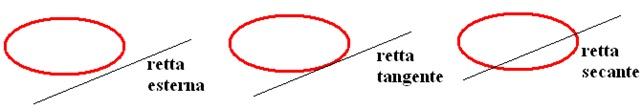
\includegraphics[width=\textwidth]{img/rettaconica.jpg}
  \caption{Posizioni reciproche tra una retta ed un'ellisse.}%
  %\label{fig:ellissedalcono}
  %    \end{inaccessibleblock}
\end{figure}
Geometricamente per stabilire la posizione di una retta rispetto ad una 
conica, disegniamo i due oggetti sul piano cartesiano e verifichiamo quanti 
punti hanno in comune. Algebricamente, per stabilire la posizione di una 
retta rispetto ad una conica andiamo a considerare il sistema delle due 
equazioni, quella della conica, ad esempio un'ellisse e quella della 
retta:

$\begin{cases}  \dfrac{x^{2}}{a^{2}}+\dfrac{y^{2}}{b^{2}}=1   \\ y=mx+q  
\end{cases}$

Il sistema si sviluppa in un'equazione di secondo grado nella quale il 
segno del $\Delta$ determina, la posizione reciproca fra retta ed ellisse:
\begin{itemize}
  \item se $\Delta$<0, l'equazione di secondo grado non ha soluzioni 
reali e dunque retta e conica non hanno punti in comune, non si intersecano;
  \item se $\Delta$=0, l'equazione di secondo grado, deducibile dal 
sistema, ha due soluzioni coincidenti e quindi conica e retta hanno un solo 
punto in comune: la retta è tangente alla conica;
  \item se $\Delta$>0, l'equazione di secondo grado ha due soluzioni 
e di conseguenza i punti in comune tra retta e conica sono due: la retta è 
secante alla conica.
\end{itemize}
In generale per determinare le intersezioni tra una retta e una conica, 
trovando così la posizione relativa della retta rispetto alla conica, 
dobbiamo risolvere un sistema a due equazioni, quella della conica e quella 
della retta. 

Per fare una ulteriore applicazione studiamo le intersezioni tra una 
parabola e una retta.
Data la parabola di equazione P: y=a$ x^{2}+bx+c$ e la retta generica $r$: 
y=mx+q le loro intersezioni sono determinate dal sistema:

$\begin{cases}  y=a x^{2} +bx+c   \\ y=mx+q  
\end{cases}$

dal quale otteniamo l'equazione:
$ax^{2} +(b-m)x+c-q=0$
equazione di secondo grado in x, le cui soluzioni sono le ascisse dei punti 
di intersezione, a seconda del segno del $ \Delta $ dell'equazione ci 
saranno due soluzioni nel caso di retta secante, una nel caso di retta 
tangente e nessuna nel caso di retta esterna, come mostrato nela seguente 
figura:
\begin{figure}[htbp]
  \centering
  %    \begin{inaccessibleblock}[Cono a due falde tagliato da un piano
  %      che forma un'ellisse.]
  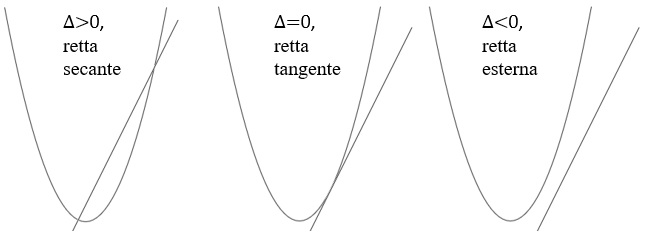
\includegraphics[scale=0.6]{img/rettaconica3.jpg}
  \caption{Posizioni reciproche tra una retta ed una parabola.}%
  %\label{fig:ellissedalcono}
  %    \end{inaccessibleblock}
\end{figure}

\begin{esempio} Data l'ellisse $ \dfrac{x^{2}}{16}+  
\dfrac{y^{2}}{4} =1$ e la retta $y=x+4$, stabilire la posizione della retta 
rispetto all'ellisse e le coordinate degli eventuali punti di intersezione. 
Secondo quanto visto il sistema da risolvere è:

$\begin{cases}  \dfrac{x^{2}}{16}+\dfrac{y^{2}}{4}=1   \\ y=x+4  
\end{cases}$  
sostituendo otteniamo l'equazione: $ 
\dfrac{x^{2}}{16}+\dfrac{x^{2}+8x+16}{4}=1$ che semplificata risulta: $5 
x^{2} +32x+48=0$.
con $ \Delta =64>0$. 

\begin{minipage}{.65\textwidth}
  La retta è dunque secante, calcoliamo ora i due punti di 
intersezione. 
  Risolvendo l'equazione otteniamo le ascisse dei punti di 
intersezione $ x_{1} =- \dfrac{12}{5} $ e $ x_{2} =-4$. Sostituendo tali 
ascisse nell'equazione della retta otteniamo le corrispondenti ordinate $ 
y_{1} =\dfrac{8}{5}$ e $ y_{2} =0$. I punti cercati sono $ P_{1}  
\left(-\dfrac{12}{5};~ \dfrac{8}{5}\right) $ e $ P_{2} =(-4;~0)$.
\end{minipage}
\hspace{.2cm}
\begin{minipage}{.3\textwidth}
  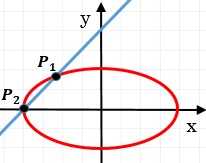
\includegraphics[width=\textwidth]{img/esempioposizione1.jpg}
  %    \caption{Generazione di un cono a due falde}% 
\end{minipage}
\end{esempio}
 
\section{Rette tangenti ad una conica}
Analizziamo ora, nello specifico, il caso di tangenza. In generale, per un 
punto esterno ad una conica possono esser condotte due tangenti mentre per 
un punto appartenente alla conica può essere condotta una sola tangente;  
da un punto interno alla conica, cioè dalla sua parte convessa, non si 
possono tracciare tangenti, come illustrato di seguito nel caso della 
parabola. 

\begin{figure}[t]
  \centering
  %    \begin{inaccessibleblock}[Cono a due falde tagliato da un piano
  %      che forma un'ellisse.]
  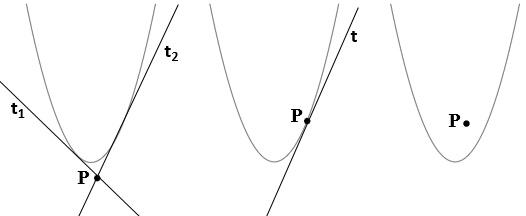
\includegraphics[scale=0.8]{img/tangenti2.jpg}
  \caption{Rette tangenti alla parabola.}%
  %\label{fig:ellissedalcono}
  %    \end{inaccessibleblock}
\end{figure}

Quanto appena visto per la parabola vale anche per le altre coniche.
Vogliamo ora determinare le rette tangenti ad una conica passanti per un 
punto dato. I casi possibili, come abbiamo appena visto, sono due: se il 
punto è esterno alla conica, in generale, si trovano due rette tangenti, se 
il punto appartiene alla conica, una sola tangente.

\textbf{A) Determinazione delle tangenti ad una conica passanti per un 
punto dato P($ x_{0}$; $ y_{0}$) esterno ad essa}.
Per un punto esterno ad una conica passano due rette tangenti alla conica 
stessa. Per determinare le equazioni di queste tangenti, conoscendo la 
conica e le coordinate del punto esterno, in generale, si procede con il 
metodo del $ \Delta $=0. Andiamo ad illustrare per punti tale metodo:
\begin{itemize}
  \item si scrive l'equazione del fascio di rette proprio centrato 
nel punto dato, avente m variabile: $y- y_{0} =m\left(x-x_{0}\right)$;
  \item si mette a sistema tale equazione con quella della conica 
data;
  \item si risolve il sistema per una variabile, x o y, trovando una 
equazione di secondo grado ad un parametro (m) e si determina il $ \Delta $ 
di tale equazione;
  \item ponendo $ \Delta $=0 si determinano i valori del parametro m 
che costituiscono i coefficienti angolari delle rette tangenti cercate, che 
si determinano sostituendo tali m trovati nell'equazione del fascio di 
rette iniziale.
\end{itemize}

  Poniamo attenzione a quest'ultimo punto, infatti, se l'equazione 
del $ \Delta $ è di secondo grado in m, i due m rappresentano i due 
coefficienti angolari delle due rette, se l'equazione del $ \Delta $ è di 
primo grado la sua soluzione rappresenterà il coefficiente di una retta 
tangente mentre l'altra tangente sarà fornita dalla retta verticale $x= 
x_{0} $. 

  Nella formula del fascio di rette infatti non è mai compresa la 
retta verticale passante per il centro del fascio, tale retta, per 
completare il fascio, va aggiunta alla formula del fascio:
  $y-y_{0} =m(x- x_{0} ) \cup x= x_{0} $
  

\begin{esempio} Determinare le equazioni delle tangenti 
all'ellisse $ x^{2} + \dfrac{y^{2}}{3} $=1 condotte dal punto $P(2;~0)$.

Procediamo come appena indicato. L'equazione del fascio di rette di centro 
P è $y-0=m(x-2)~ U ~x=2$, il sistema che otteniamo, mettendo insieme conica 
data e fascio appena determinato, è:

$\begin{cases}  x^{2}+\dfrac{y^{2}}{3}=1   \\ y=mx-2m  
\end{cases}$  
$\begin{cases}  3x^{2}+y^{2}=3   \\ y=mx-2m  
\end{cases}$
$\begin{cases}  3x^{2}+m^{2}x^{2}+4m^{2}-4m^{2}x-3=0   \\ y=mx-2m  
\end{cases}$

riscriviamo l'equazione di secondo grado ottenuta, trovandone il $ \Delta $ 
con la formula ridotta: (3+$ m^{2} $)$ x^{2} $-4$ m^{2} $x+4$ m^{2} $-3=0, 
$ \Delta $=4$ m^{4} $-(3+$ m^{2} $)(4$m^{2}$-3)=4$ m^{4} $-12$ m^{2} $+9-4$ 
m^{4} $+3$ m^{2} $=-9$ m^{2} $+9. Ponendo il $ \Delta $=0 e risolvendo 
l'equazione pura che si trova abbiamo $ m_{1} $=1 e $ m_{2} $=-1.

Sostituiamo gli m appena trovati nell'equazione del fascio per trovare le 
rette tangenti: y=x-2 e y=-x+2.
\end{esempio}

\begin{esempio} Determinare le equazioni delle tangenti 
all'ellisse $ x^{2} $+$ \dfrac{y^{2}}{3} $=1 condotte dal punto P(1; 2).

L'equazione del fascio di rette di centro P è y-2=m(x-1) U x=1, il sistema 
che otteniamo, mettendo insieme conica data e fascio appena determinato è:

$\begin{cases}  x^{2}+\dfrac{y^{2}}{3}=1   \\ y=mx-m+2  
\end{cases}$  
$\begin{cases}  3x^{2}+y^{2}=3   \\ y=mx-m+2  
\end{cases}$
$\begin{cases}  3x^{2}+m^{2}x^{2}+m^{2}+4-2m^{2}x-4m+4mx-3=0   \\ y=mx-m+2  
\end{cases}$

l'equazione di secondo grado risulta: $\left(3+ m^{2} \right) x^{2} 
+2\left(2m-m^{2} \right)x+ m^{2} -4m+1=0$ e il $ \Delta $ della formula 
ridotta è $ \Delta =4 m^{2} + m^{4} -4 m^{3} -\left(3+ m^{2} \right)\left( 
m^{2}-4m+1 \right)=4 m^{2} + m^{4} -4 m^{3} -3 m^{2} +12m-3- m^{4} +4 m^{3} 
- m^{2} =12m-3$. Ponendo ora $ \Delta =0$, otteniamo che $m=\dfrac{1}{4}$. 
Essendo il $ \Delta $ di primo grado il possibile m, coefficiente angolare, 
è soltanto uno e la corrispondente retta risulta $y-2=\dfrac{1}{4}(x-1)  
\longrightarrow  4y-x-7=0$. L'altra retta tangente è la retta verticale 
passante per il punto P: x=1.
\end{esempio}

\textbf{B) Determinazione della tangente ad una conica passante per un 
punto dato $P( x_{0}; ~ y_{0})$ appartenente alla conica}.

Se il punto, per il quale si vogliono cercare le tangenti ad una conica, 
appartiene alla conica, necessariamente si troverà una sola retta tangente. 
Per trovare tale retta si può ricorrere ancora al metodo precedente del 
sistema tra conica e fascio di rette, ponendo poi il $ \Delta $=0, ma si 
preferisce, in questo caso, usare il meno complesso metodo dello 
sdoppiamento. Tale metodo evita di impostare e risolvere il sistema a due 
equazioni di secondo grado e con una semplice sostituzione si trova 
immediatamente la retta tangente cercata.
Andiamo ad illustrare per punti tale metodo, utilizzando come esempio di 
conica una circonferenza, ma sottolineando subito che tale metodo può 
essere applicato ad una qualsiasi conica:

\begin{itemize}
  \item   dato il punto $P( x_{0};~ y_{0} )$ appartenente alla 
circonferenza e scritta l'equazione canonica della circonferenza $ x^{2} + 
y^{2} +ax+by+c=0$ si procede con la seguente sostituzione:

  $ x^{2} \longrightarrow x x_{0} $;  $ y^{2} \longrightarrow y y_{0} 
$;  $x= \dfrac{x+x_{0}}{2} $;  $y= \dfrac{y+y_{0}}{2} $
  ;
  \item otteniamo la seguente equazione che rappresenta la retta 
tangente cercata:

  $x x_{0} +y y_{0}+a \dfrac{x+x_{0}}{2}  +b \dfrac{y+y_{0}}{2} +c=0$
\end{itemize}

\begin{esempio} Determinare l' equazione della tangente 
all'ellisse $ \dfrac{x^{2}}{25}+\dfrac{y^{2}}{36} =1$ passante per il suo 
punto $P\left(3; ~-\dfrac{24}{5}\right)$. 
Procediamo come appena indicato, mediante il metodo dello sdoppiamento. 
Applichiamo le sostituzioni appena viste:\\ $ \dfrac{xx_{0}}{25} +
 \dfrac{yy_{0}}{36} =1  \longrightarrow  \dfrac{3x}{25} -  \dfrac{24y}{5 
\cdot 36} =1  \longrightarrow  \dfrac{108x-120y}{900}=\dfrac{900}{900} 
\longrightarrow 9x-10y-75=0$.
\end{esempio}

\section{Curve deducibili dalle equazioni delle coniche}

La conoscenza delle equazioni e delle proprietà delle coniche consente di 
rappresentare graficamente alcune tipologie di funzioni irrazionali.\\ 
Vediamone un esempio: tracciamo il grafico della funzione 
$y=\sqrt{4-9x^{2}}$. Innanzitutto la funzione è definita solo se il 
radicando è non negativo, cioè se $4-9x^{2}\geq0$ e questa disequazione è 
risolta per $ -\dfrac{2}{3}\leq x\leq \dfrac{2}{3}$. il secondo membro 
dell'equazione risulta così non negativo e per mantenere l'uguaglianza 
anche il primo membro deve essere non negativo, otteniamo dunque $ y\geq0 $. 
Ora con le condizioni poste possiamo elevare al quadrato entrambi i membri 
per eliminare la radice, ottenendo $ y^{2}=4-9x^{2} $ che non è altro che 
l'equazione di un'ellisse: $ 9x^{2}+y^{2}=4 $.\\ Quanto appena visto 
equivale all'impostazione del sistema:\\
$\begin{cases}  4-9x^{2}\geq0   \\ y\geq0  \\y^{2}=4-9x^{2} 
\end{cases}$  
$\begin{cases}   -\dfrac{2}{3}\leq x\leq \dfrac{2}{3}   \\ y\geq0  \\ 
9x^{2}+y^{2}=4 
\end{cases}$  

\begin{figure} [h]
  \noindent \begin{minipage}{.75\textwidth}
    La soluzione grafica di questo sistema è un'ellisse che ha 
dei limiti sia in ascissa che in ordinata, per tener conto di $ y\geq0 $ 
dobbiamo prendere solo la parte dell'ellisse con orinata positiva o nulla, 
cioè la parte di ellisse contenuta nel primo e secondo quadrante; teniamo 
conto dei limiti sulle ascisse considerando le condizioni di esistenza del 
radicale, cioè la soluzione della prima equazione del sistema. Graficamente 
otteniamo la figura qui a fianco.
  \end{minipage}
  \hspace{0.5cm}
  \begin{minipage}{.2\textwidth}
    %    \begin{inaccessibleblock}[Cono a due falde tagliato da un piano
    %      che forma un'ellisse.]
    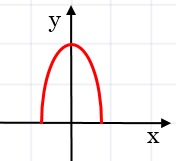
\includegraphics[width=\textwidth]{img/curva1.jpg}
    \caption{Grafico dell'equazione $ y=\sqrt{4-9x^{2}} $.}
    %\label{fig:ellissedalcono}
    %    \end{inaccessibleblock} 
  \end{minipage}
\end{figure}
Consideriamo un altro esempio: $y=2-\sqrt{6x-x^{2}}  $ e proviamo a 
disegnarne il grafico corrispondente. Come primo passo riscriviamo la 
funzione come $y-2=-\sqrt{6x-x^{2}}  $, poi cerchiamo di impostare un 
sistema simile al precedente che rispetti le condizioni di esistenza del 
radicale e le sue conseguenze:\\
$\begin{cases}  6x-x^{2}\geq0   \\ y-2\leq0  \\y^{2}-4y+4=6x-x^{2} 
\end{cases}$  
$\begin{cases}   0\leq x\leq6   \\ y\leq2  \\ x^{2}+y^{2}-6x-4y+4=0 
\end{cases}$   \\ \\ \\ \\ \\
\begin{figure} [h]
  \noindent \begin{minipage}{.75\textwidth}
    La prima equazione rappresenta di nuovo le condizioni del 
radicale, la seconda equazione ci ricorda che il primo membro, y-2, deve 
avere lo stesso segno del secondo, che essendo una radice con il segno 
negativo davanti, non può essere positivo, infine la terza rappresenta 
l'elevamento al quadrato dei due membri ed identifica una circonferenza di 
centro (3; 2) e raggio 3. Il grafico cercato è dunque quello di una 
circonferenza con le caratteristiche trovate limitata nelle ordinate a 
$y\leq2$ e nelle ascisse a $ 0\leq x\leq6 $.
  \end{minipage}
  \hspace{0.5cm}
  \begin{minipage}{.2\textwidth}
    %    \begin{inaccessibleblock}[Cono a due falde 
tagliato da un piano
    %      che forma un'ellisse.]
    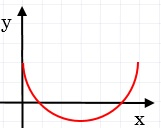
\includegraphics[width=\textwidth]{img/curva2.jpg}
    \caption{Grafico dell'equazione $ y=2-\sqrt{6x-x^{2}} $.}
    %\label{fig:ellissedalcono}
    %    \end{inaccessibleblock} 
  \end{minipage}
\end{figure}
\begin{figure} [h]
  \noindent \begin{minipage}{.75\textwidth}
    Ancora un esempio che riguarderà stavolta la parabola. 
Vogliamo disegnare il grafico di $ y=\sqrt{4-x} $, il sistema 
corrispondente è:

    $\begin{cases}  4-x\geq0   \\ y\geq0  \\y^{2}=4-x 
    \end{cases}$  
    $\begin{cases}   x\leq4   \\ y\geq0  \\ x=-y^{2}+4 
    \end{cases}$ 
    
otteniamo una parabola con l'asse parallelo all'asse Y e di questa parabola 
prendiamo in considerazione solo la parte con y non negativa.
  \end{minipage}
  \hspace{0.5cm}
  \begin{minipage}{.2\textwidth}
    %    \begin{inaccessibleblock}[Cono a due falde 
tagliato da un piano
    %      che forma un'ellisse.]
    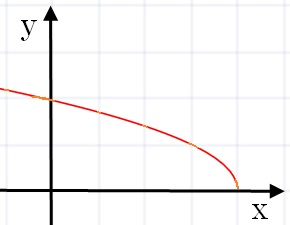
\includegraphics[width=\textwidth]{img/curva3.jpg}
    \caption{Grafico dell'equazione $ y=\sqrt{4-x} $.}
    %\label{fig:ellissedalcono}
    %    \end{inaccessibleblock} 
  \end{minipage}
\end{figure}

\section{Esercizi}

\subsection{Esercizi dei singoli paragrafi}

Posizioni di una retta rispetto ad una conica
\begin{esercizio}
  \label{ese:div.003}
  Considera la conica data e stabilisci se le rette al suo fianco 
sono secanti, tangenti od esterne.
  \begin{enumeratea}

\item $y=3 x^{2} +6x-4;~r:~y=2x+3,~s:~y=\dfrac{1}{4}x-8,~t:~y=-3x-1$\\ 
\hfill  $\left[r~secante,~s ~esterna,~ t~secante\right]$
\item $y=-x^{2}+2x+4;~r:~y=4x+5,~s:~y=3x+1,~t:~y=-2x+8$\\
\hfill $\left[r~tangente,~s~esterna,~t~tangente\right]$
\item $\dfrac{x^{2}}{18} 
+\dfrac{y^{2}}{36}=1;~r:~y=3x-2,~s:~y=-6,~t:~y=-2x+8$\\
\hfill $\left[r~secante,~s~tangente,~t~esterna\right]$
\item $\dfrac{x^{2}}{25}+\dfrac{y^{2}}{4}=1;~r:~y=-2x+1,~s:~y=3x,~t:~y= 
\dfrac{x}{2} +6$\\
\hfill $\left[r~secante,~s~secante,~t~esterna\right]$
\item $ x^{2}+y^{2}=4;~r:~y=-x-1,~s:~y=x+3,~t:~x+\sqrt{3}y=4$\\
\hfill $\left[r~secante,~s~esterna,~t~tangente\right]$
\item $4 x^{2}-5 y^{2}=20;~r:~y=~-x-1,~s:~y=3x,~t:~y=3x+7$\\
\hfill $\left[r~tangente,~s~esterna,~t~secante\right]$
\item $\dfrac{x^{2}}{9}-\dfrac{y^{2}}{4}=1;~r:~5x-6y-9=0,~s:~x=4,~t:~ 
x-3y-3=0$\\
\hfill $\left[r~tangente,~s~secante,~t~secante\right]$
\item $x^{2}+y^{2}-4x+2y=0;~r:~x+2y-5=0,~s:~x+4y-5=0,~t:~-x+2y-8=0$\\
\hfill $\left[r~tangente,~s~secante,~t~esterna\right]$
\end{enumeratea}
\end{esercizio}

\begin{esercizio}
  \label{ese:div.003}
  Determina i punti di intersezione tra le coniche e le rette 
sottostanti, dopo aver verificato che la retta è tangente alla conica.
  \begin{enumeratea}
  \item $ x^{2}+4y^{2}=1 $, $y=x+1$
  \hfill$\left[P_{1}\left( -\dfrac{3}{5};~\dfrac{2}{5} \right);~ 
P_{2}\left(-1;~0\right)\right]$
  \item  $4x^{2}+y^{2}=4 $, $y=x+2$
  \hfill$\left[P_{1}\left( -\dfrac{4}{5};~\dfrac{6}{5} \right);~ 
P_{2}\left(0;~2\right)\right]$
  \item $5x^{2}-y^{2}=11 $, $y=2$
  \hfill$\left[P_{1}\left( \sqrt{3};~2 \right);~ 
P_{2}\left(-\sqrt{3};~2\right)\right]$
  \item $9x^{2}-25y^{2}=225 $, $y=\dfrac{2}{5}x+2$
  \hfill $\left[P_{1}\left(13;~\dfrac{36}{5} \right);~ 
P_{2}\left(-5;~0\right)\right]$
  \end{enumeratea}
\end{esercizio}
Rette tangenti ad una conica

\begin{esercizio}
  \label{ese:div.003}
  Determina le rette tangenti alla conica indicata passanti per il 
punto A, ad essa esterno.
  \begin{enumeratea}

\item $9x^{2}+4y^{2}=36,~A(2;~5)$  
\hfill $\left[y=\dfrac{4}{5}x+\dfrac{17}{5};~x=2\right]$
\item $x^{2}+2y^{2}=2,~A(2;~1)$
\hfill $\left[y=1;~y=2x+3\right]$
\item $\dfrac{x^{2}}{4}+\dfrac{y^{2}}{5}=1,~A(3;~0)$
\hfill $\left[y=-x+3;~y=x-3\right]$
\item $\dfrac{x^{2}}{16}+\dfrac{y^{2}}{9}=1,~A(6;~-1)$
\hfill $\left[y=-x+5;~y=\dfrac{2}{5}x-\dfrac{17}{5}\right]$
\item $\dfrac{x^{2}}{9}-\dfrac{y^{2}}{4}=1,~A(0;~3)$
\hfill $\left[y=-\dfrac{6}{5}x+3;~y=\dfrac{6}{5}x+3\right]$
\item $\dfrac{x^{2}}{25}-\dfrac{y^{2}}{16}=1,~A(-5;~-2)$ 
\hfill $\left[x=-5;~y=x+3\right]$
\item $x^{2}-2y^{2}=2,~A(1;~2)$
\hfill $\left[y=-5x+7;~y=x+1\right]$
\item $4x^{2}-9y^{2}=144,~A(0;~2)$
\hfill $\left[y=\dfrac{3}{4}x+2;~y=-\dfrac{3}{4}x+2\right]$
\end{enumeratea}
\end{esercizio}

\begin{esercizio}
  \label{ese:div.003}
  Applicando la formula dello sdoppiamento determina la tangente alla 
conica data passante per il suo punto A.
  \begin{enumeratea}
\item $\dfrac{x^{2}}{4}+\dfrac{y^{2}}{9}=1,~A\left(-\dfrac{8}{5};~- 
\dfrac{9}{5}\right)$  
\hfill $\left[y=-2x-5\right]$
\item $\dfrac{x^{2}}{25}+\dfrac{y^{2}}{16}=1,~A\left(-3;~\dfrac{16}{5} 
\right)$
\hfill $\left[y=\dfrac{3}{5}x+5\right]$
\item $x^{2}+3y^{2}=3,~A\left(\dfrac{3}{2};~\dfrac{1}{2} \right)$
\hfill $\left[y=-x+2\right]$
\item $x^{2}+9y^{2}=9,~A(0;~-1)$
\hfill $\left[y=-1\right]$
\item $\dfrac{x^{2}}{9}-\dfrac{y^{2}}{4}=1,~A\left(3\sqrt{2};~2\right)$
\hfill $\left[y=\dfrac{2\sqrt{2}}{3}x-2\right]$
\item $2x^{2}-y^{2}=2,~A(3;~4)$
\hfill $\left[y=\dfrac{3}{2}x-\dfrac{1}{2}\right]$
\item $4x^{2}-3y^{2}=4,~A(2;~2)$
\hfill $\left[y=\dfrac{4}{3}x-\dfrac{2}{3}\right]$
\item $\dfrac{5x^{2}}{16}-\dfrac{y^{2}}{4}=1,~A(2;~1)$
\hfill$\left[y=\dfrac{5}{2}x-4\right]$
\end{enumeratea}
\end{esercizio}
Curve deducibili dalle equazioni delle coniche
\begin{esercizio}
  \label{ese:div.003}
  Date le seguenti funzioni irrazionali, identificane la conica che 
ne consente di determinare il grafico e, dopo aver impostato il sistema che 
le definisce, disegnale. 
  \begin{enumeratea}
    \item $ y=\sqrt{9-x} $
    \item $y=\sqrt{4-x^{2}}  $
    \item $ y=\sqrt{9-4x^{2}} $
    \item $ y=\sqrt{4x^{2}-25} $
    \item $ y=3+\sqrt{4x-x^{2}} $
    \item $ y=\sqrt{4-\dfrac{x^{2}}{4}} $
  \end{enumeratea}
\end{esercizio}

\end{comment}


  


